\documentclass{beamer}

\useoutertheme[height=0.1\paperheight,width=0.1\paperwidth,hideothersubsections]{sidebar}
\usecolortheme{whale}
\usecolortheme{orchid}

\useinnertheme[shadow]{rounded}
\setbeamercolor{title page}{fg=blue!70,bg=blue}
\setbeamercolor{logo}{bg=blue!60}
\setbeamercolor{frametitle}{fg=black,bg=blue!60}
%\setbeamercolor{section in sidebar}{fg=red}
\setbeamercolor{block title}{bg=blue!28!white,fg=blue}
\setbeamercolor{block body}{bg=red!15!white}
\setbeamercolor{sidebar}{bg=blue!70}

\setbeamertemplate{background canvas}[vertical shading][bottom=white,top=blue!25]
\usefonttheme{serif}
\setbeamertemplate{navigation symbols}{}
\usepackage{CJKutf8}
%\usepackage{subfigure}
\usepackage{xmpmulti}
\usepackage{colortbl,dcolumn}
\graphicspath{{September/}}
\DeclareGraphicsRule{*}{mps}{*}{}

\logo{\includegraphics[width=0.1\paperwidth]{huoqiang.jpg}}
\renewcommand{\raggedright}{\leftskip=0pt \rightskip=0pt plus 0cm}
\raggedright
\def\hilite<#1>{\temporal<#1>{\color{blue!35}}{\color{magenta}}{\color{blue!75}}}

\newcolumntype{H}{>{\columncolor{blue!20}}c!{\vrule}}
\newcolumntype{H}{>{\columncolor{blue!20}}c}
\newcommand{\upcite}[1]{\textsuperscript{\cite{#1}}}
\bibliographystyle{plain}
\newcommand{\yihao}{\fontsize{30pt}{\baselineskip}\selectfont}
\newcommand{\sihao}{\fontsize{14pt}{\baselineskip}\selectfont}
\newcommand{\xiaosihao}{\fontsize{12pt}{\baselineskip}\selectfont}
\newcommand{\wuhao}{\fontsize{10.5pt}{\baselineskip}\selectfont}  
\newcommand{\xiaowuhao}{\fontsize{9pt}{\baselineskip}\selectfont} 
\newcommand{\liuhao}{\fontsize{7.875pt}{\baselineskip}\selectfont}
\newcommand{\qihao}{\fontsize{5.25pt}{\baselineskip}\selectfont}
\newcommand{\ThankYouPage}{
  \begin{frame}
    \yihao \centering \textcolor{blue}
    {Thank You!}
  \end{frame}
}

\begin{document}
\begin{CJK*}{UTF8}{gkai}
  \title{九月工作总结}
  \author[\textcolor{white}{作者 朱海文}]{作者~~\textcolor{olive}{朱海文}}
  \institute{\textcolor{violet}{摩科特医疗器械有限公司}}
  \date{\today}
  \frame{\titlepage}
  %======================================================
  \section*{目录}
  \frame{\frametitle{目录}\tableofcontents}
  %=========================================
  \section{射线能谱}
  \subsection{产生的射线能谱}
  \begin{frame}\frametitle{电子打靶产生的射线能谱}
    \vskip -0.3cm
    \begin{alertblock}{}\liuhao
      首先模拟了不同能量的电子垂直轰击钨靶产生的射线能谱及空间分布,如下图,
      然后用得到的能谱穿过不同厚度的铝、铜和钛挡板,得到穿过之后的能谱和数目,同时
      记录被挡板反射的射线能谱、挡板吸收的射线能谱,以及跟2cm厚的水层作用时,
      被水层吸收的能量、被水反射的能量及最终被探测器探测到的能量。
    \end{alertblock}
    \vskip -0.3cm
    \begin{figure}[ht]
      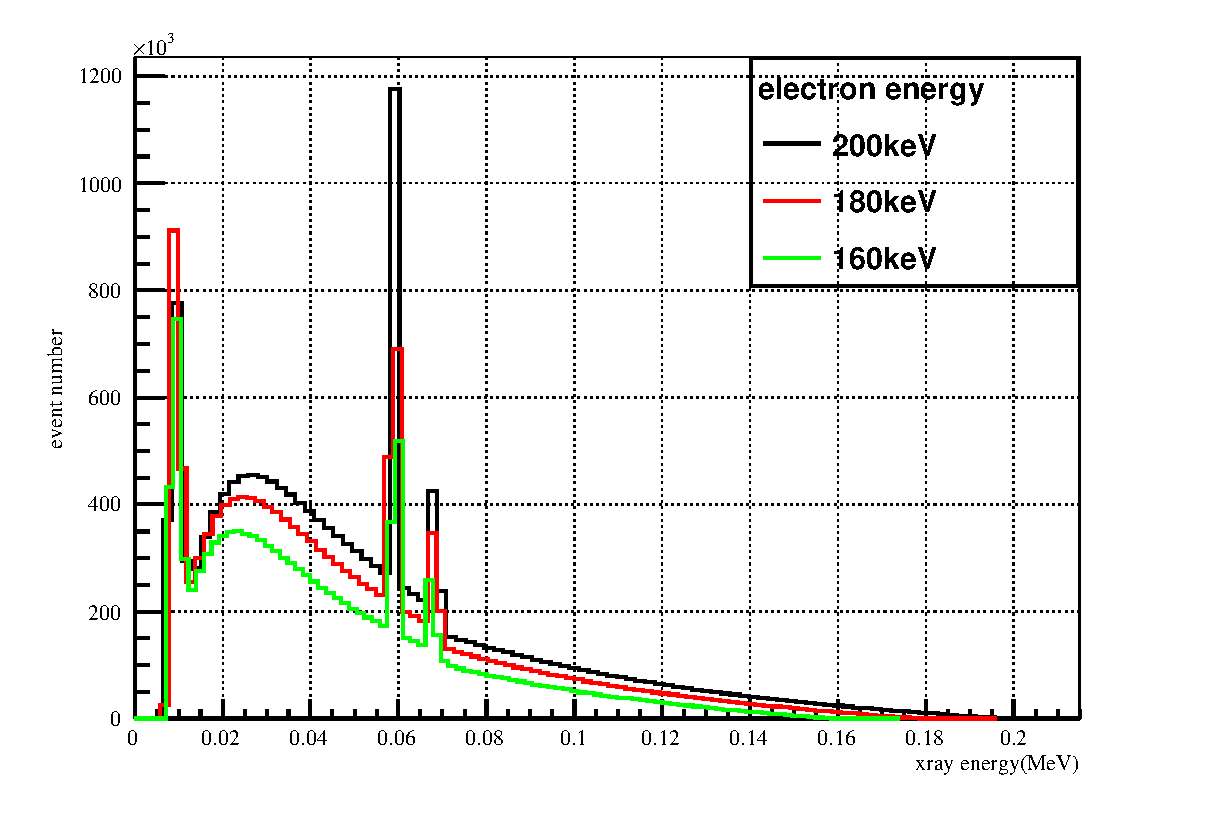
\includegraphics[width=0.45\textwidth]{xray.eps}~
      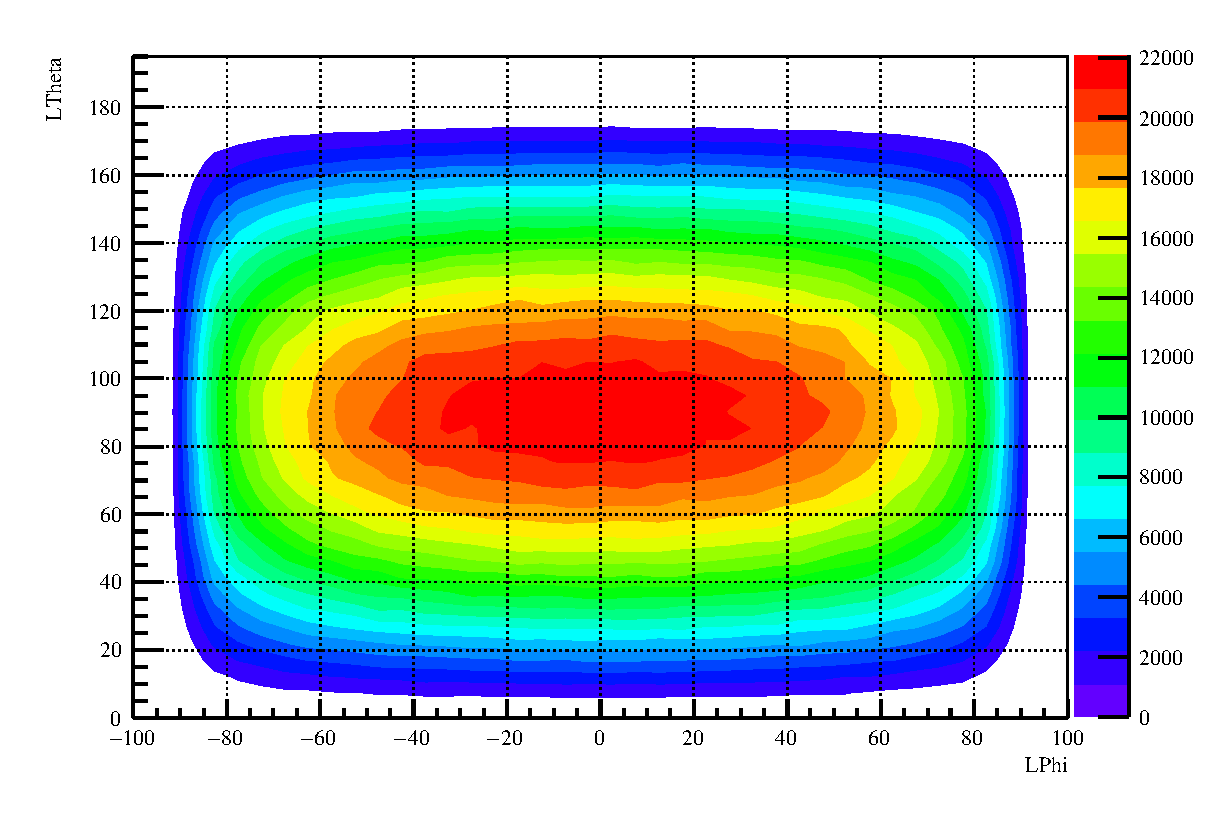
\includegraphics[width=0.45\textwidth]{xraydir.eps}

      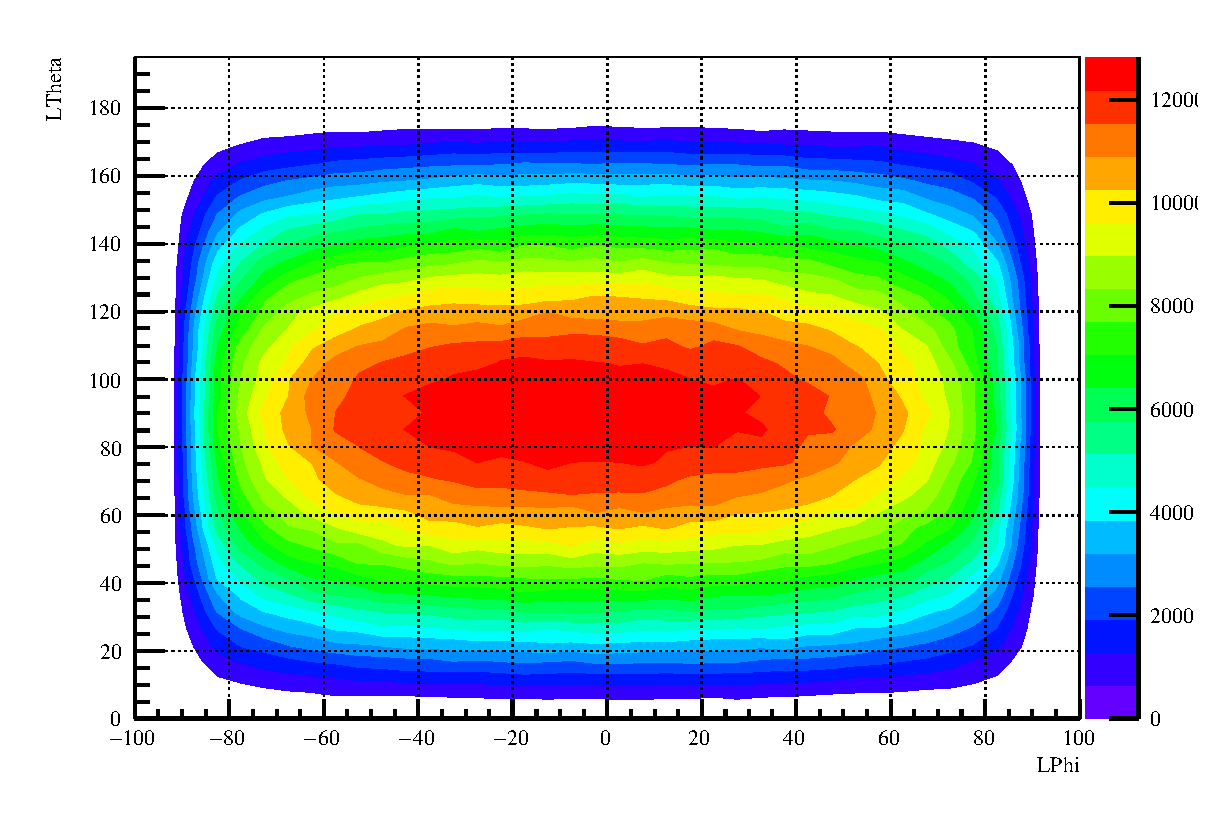
\includegraphics[width=0.45\textwidth]{Dir20dir.eps}
    \end{figure}
  \end{frame}
  %-----------------------------------
  \subsection{穿过挡板之后的能谱}
  \begin{frame}\frametitle{穿过挡板之后的能谱}
    \vskip -0.2cm
    \begin{alertblock}{\liuhao 铜挡板}
      \liuhao 下面几张图分别是200keV电子轰击钨靶产生的射线穿过不同厚度的铜片之后的能谱及各
      能量阈值下射线的比例,其他能量射线穿过其他挡板的结果跟这结果类似。
    \end{alertblock}
    \vskip -0.2cm
    \begin{figure}[ht]
      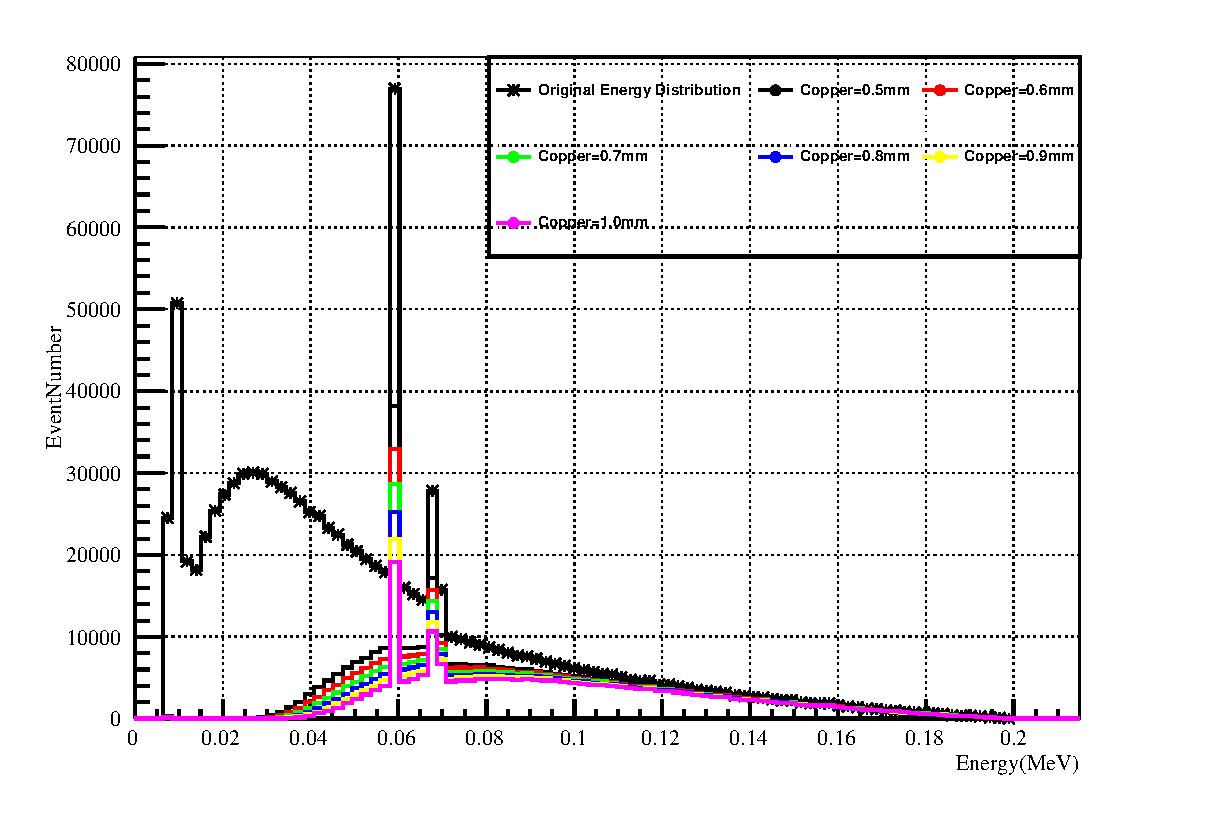
\includegraphics[width=0.5\textwidth]{200keVEnergyAfterCopperApron.eps}

      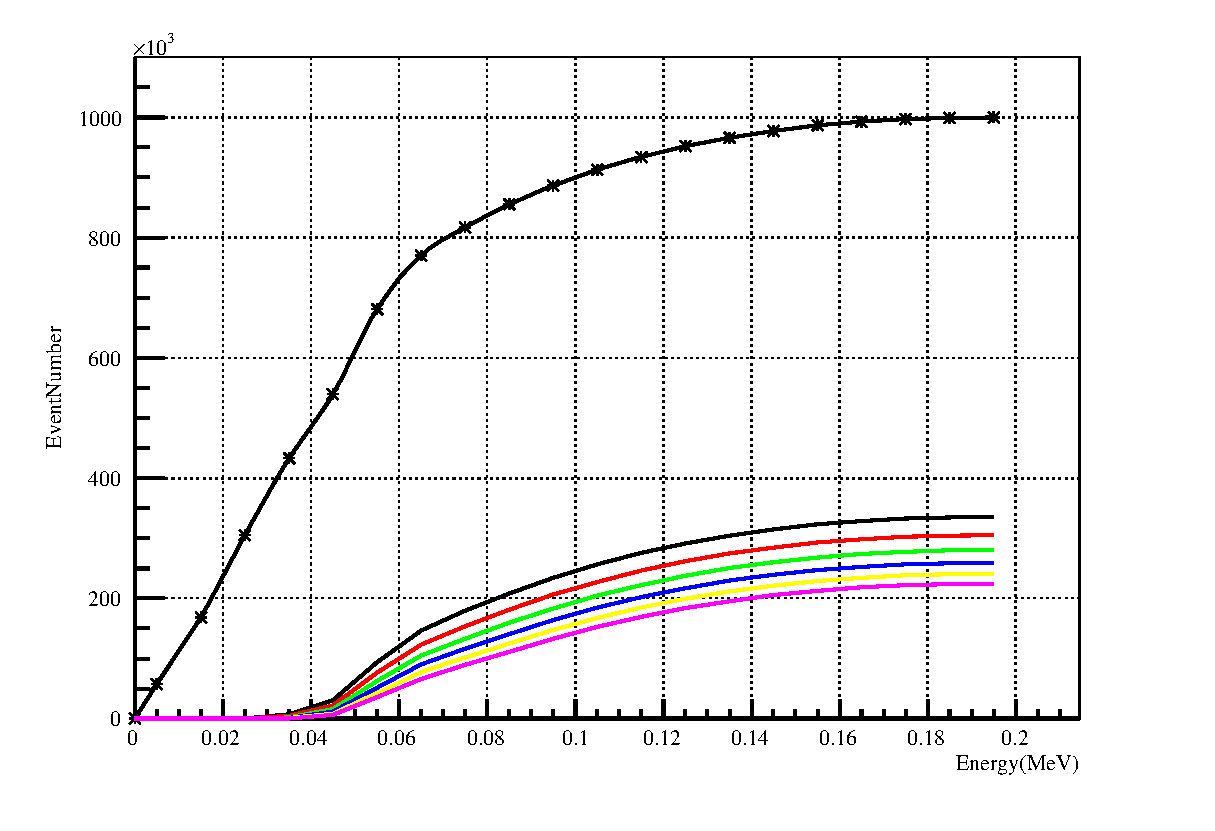
\includegraphics[width=0.45\textwidth]{200keVElectronXrayCopperDistribution.eps}~
      \includegraphics[width=0.45\textwidth]{200keVElectronXrayCopperDistributionRatio.eps}
    \end{figure}
  \end{frame}
  %-------------------------------------
  \begin{frame}\frametitle{其他能量与其他挡板}
    \vskip -0.8cm
    \begin{figure}[ht]
      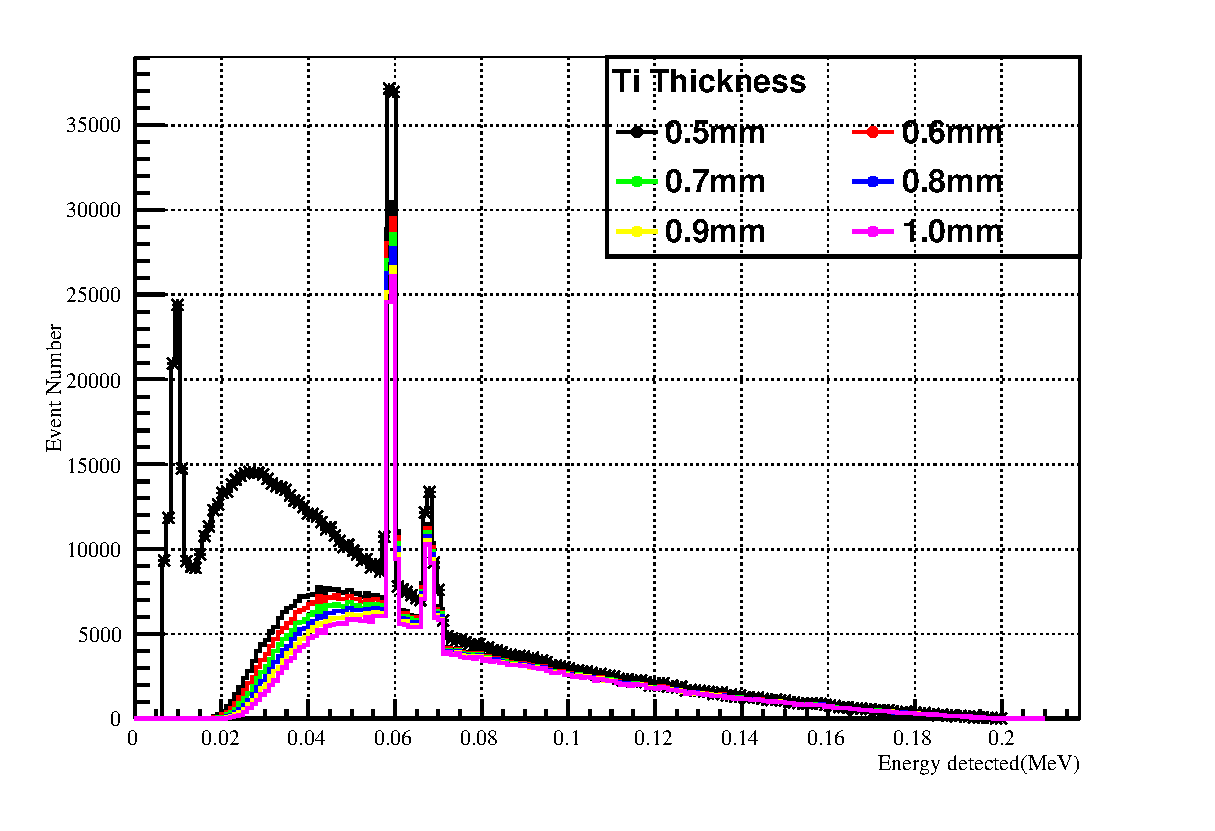
\includegraphics[width=0.33\textwidth]{EnergyAfterTiApron.eps}~
      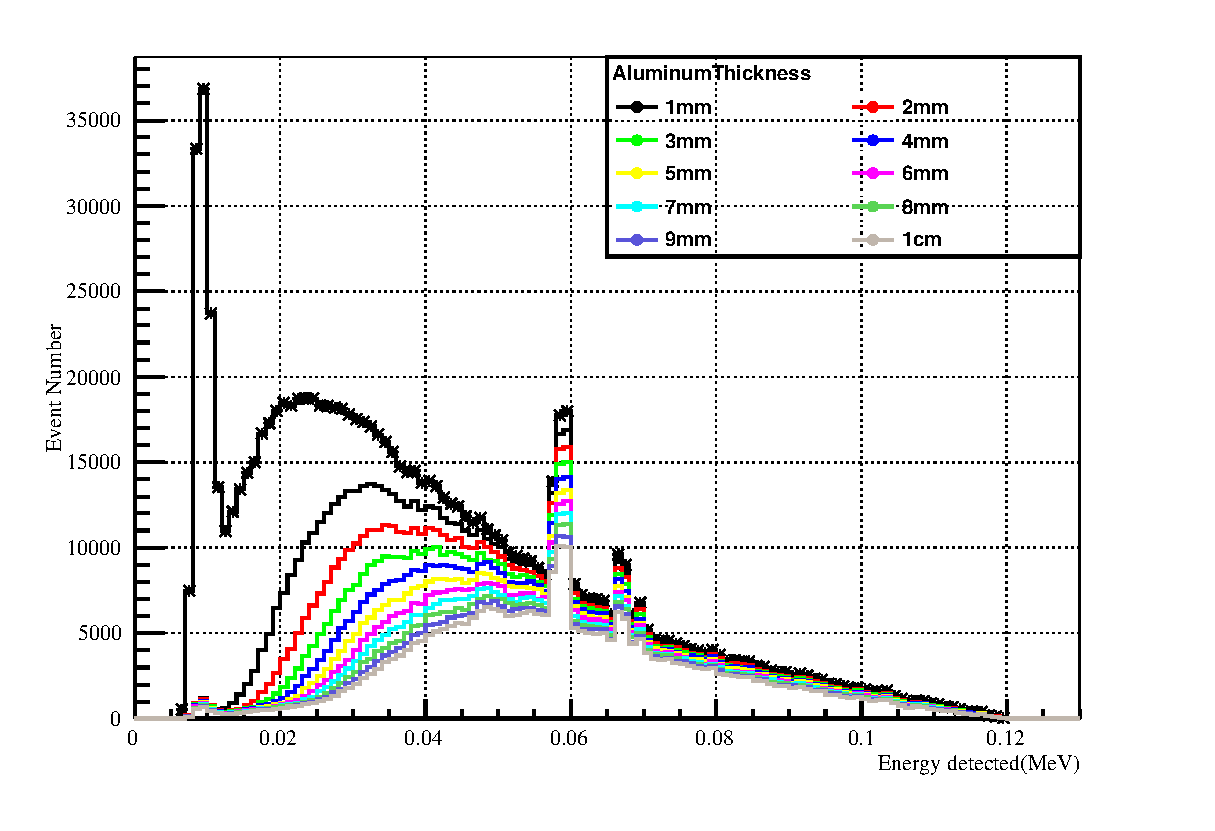
\includegraphics[width=0.33\textwidth]{EnergyAfterAluminumApron.eps}~
      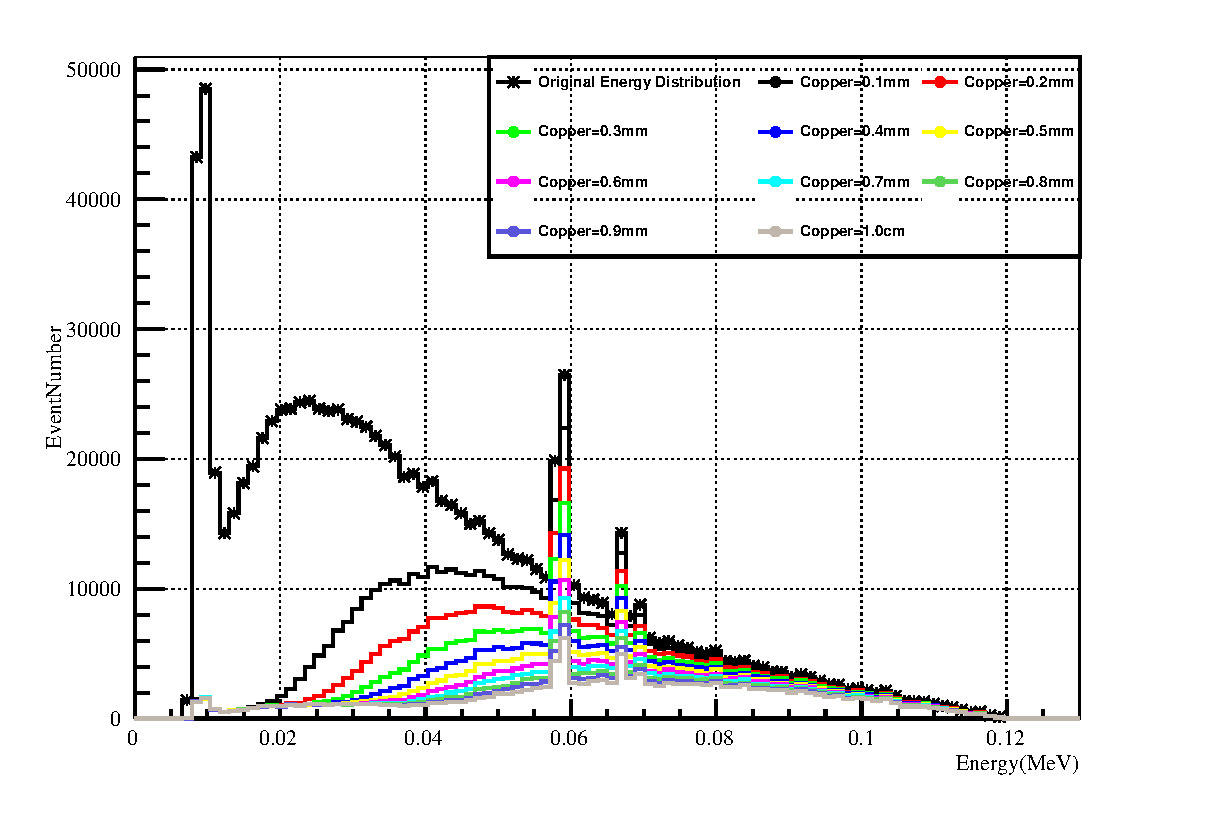
\includegraphics[width=0.33\textwidth]{EnergyAfterCopperApron.eps}

      \includegraphics[width=0.33\textwidth]{200keVElectronXrayTiDistribution.eps}~
      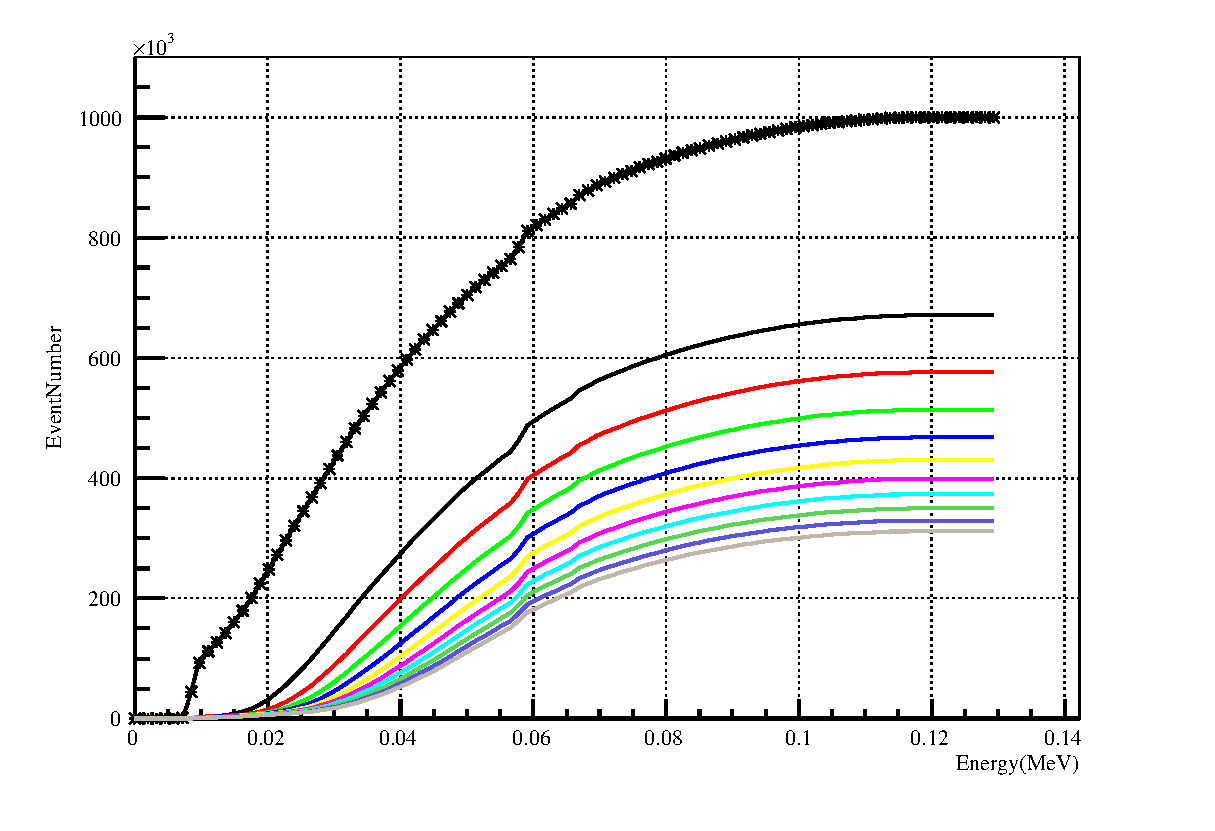
\includegraphics[width=0.33\textwidth]{AluminumDistribution.eps}~
      \includegraphics[width=0.33\textwidth]{CopperDistribution.eps}
      
      \includegraphics[width=0.33\textwidth]{180keVElectronXrayTiDistributionRatio.eps}~
      \includegraphics[width=0.33\textwidth]{AluminumDistributionRatio.eps}~
      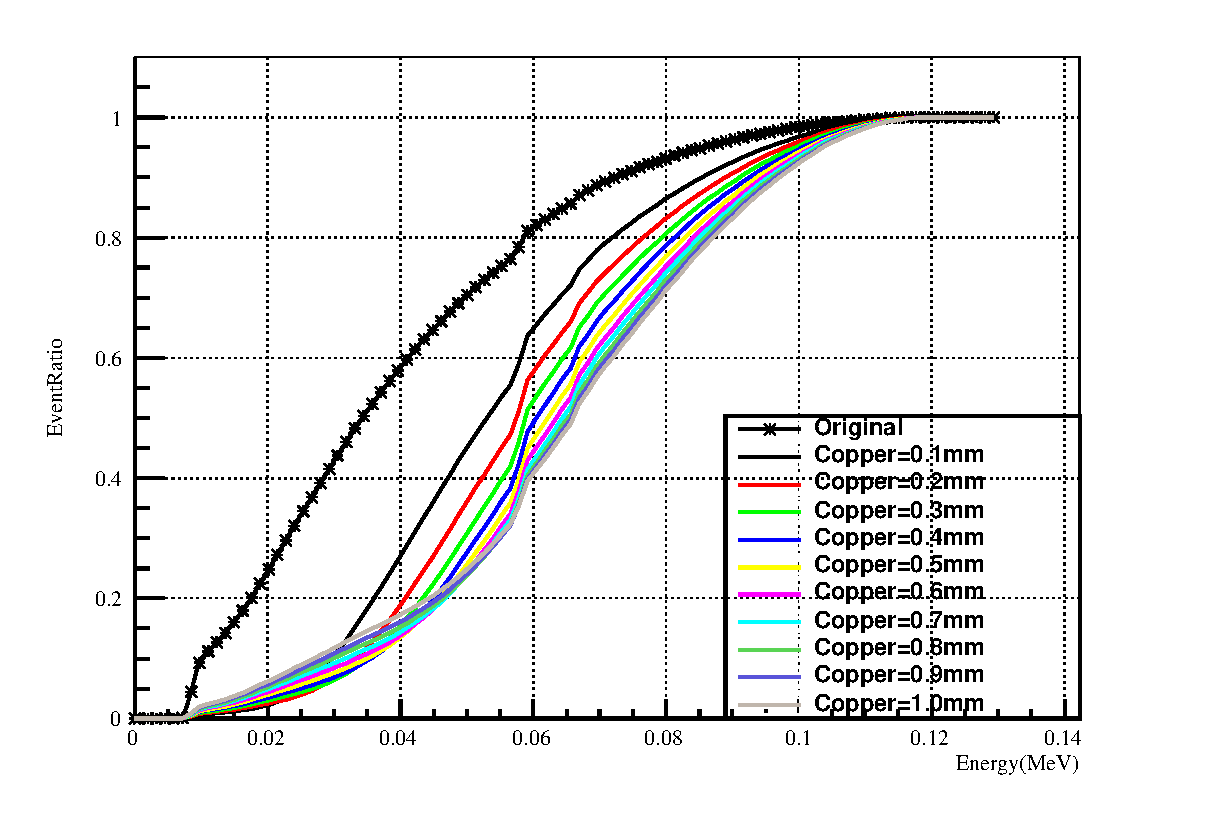
\includegraphics[width=0.33\textwidth]{CopperDistributionRatio.eps}
    \end{figure}
    \vskip -0.3cm
    \liuhao
    最后对这些数据都进行了定量的统计。
  \end{frame}
  %-----------------------------------------
  \subsection{各成分的能谱}
  \begin{frame}\frametitle{各成分的能谱}
    \begin{figure}[ht]
      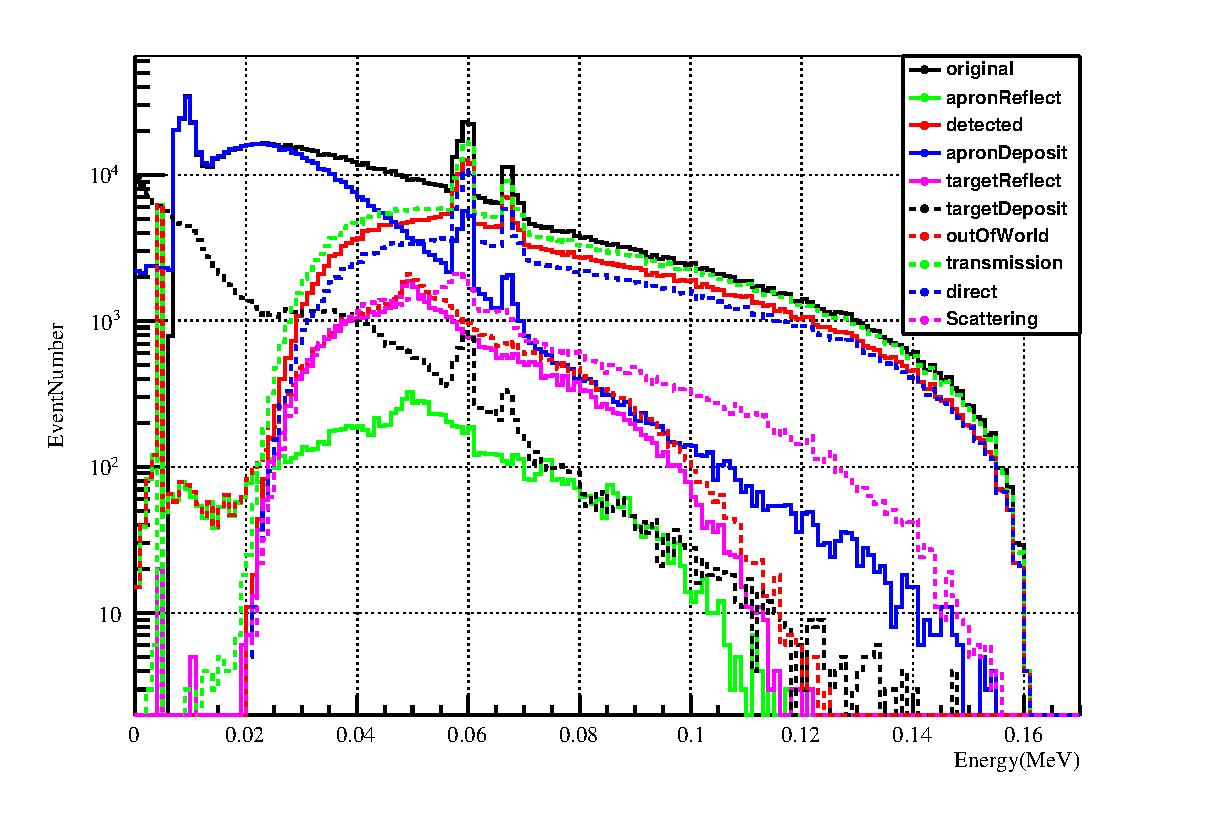
\includegraphics[width=\textwidth]{1mmTiApron160keVelectronEnergySpectrum.eps}
    \end{figure}
  \end{frame}
  %----------------
  \subsection{直射与散射}
  \begin{frame}\frametitle{直射与散射}
    \begin{figure}[ht]
      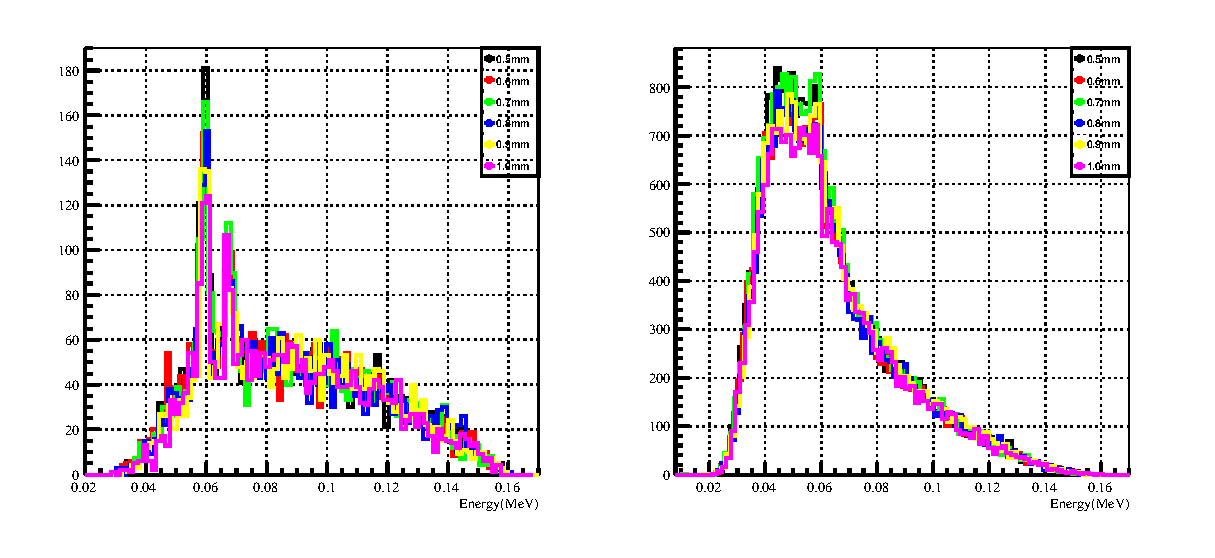
\includegraphics[width=\textwidth]{TiApron160keVelectronXraydirectandscat.eps}

      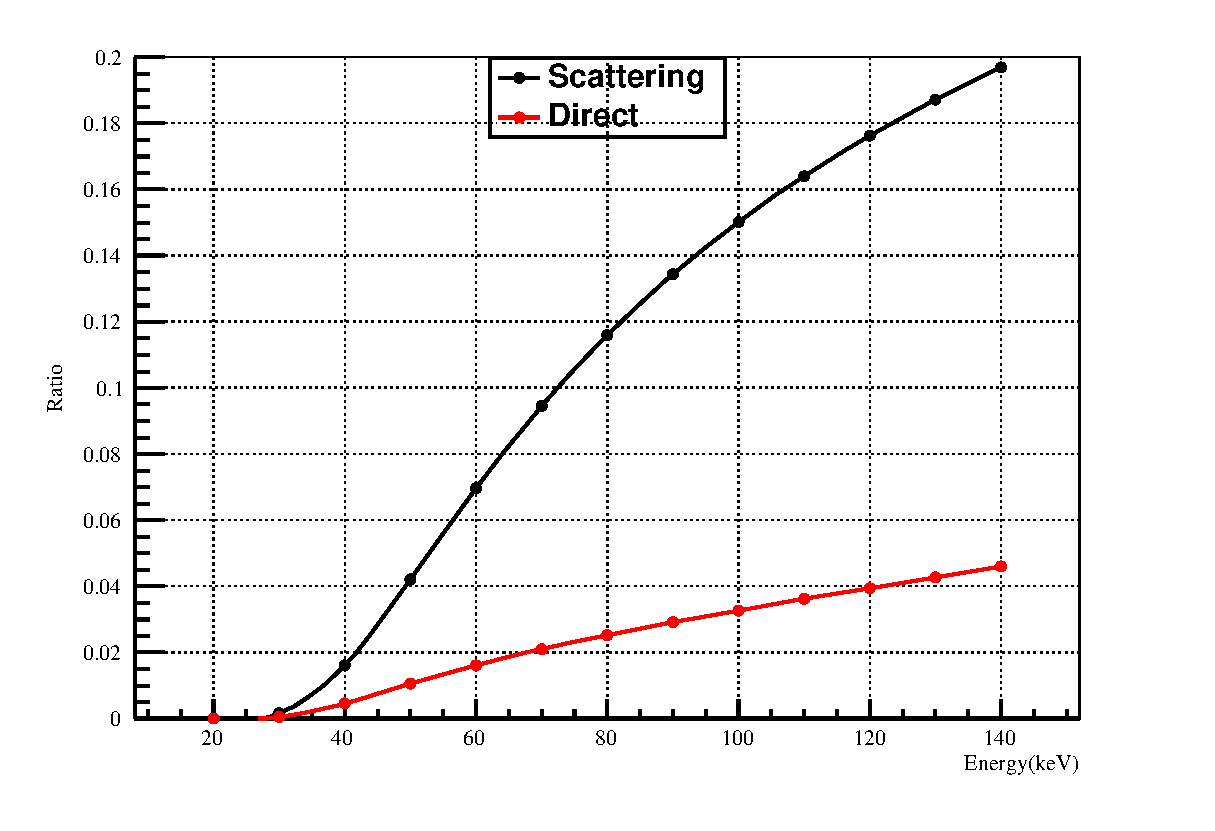
\includegraphics[width=0.45\textwidth]{ScatDirectRatio.eps}
    \end{figure}
  \end{frame}
  %=======================
  \section{学习重建算法}
  \ThankYouPage
\end{CJK*}
\end{document}
